\chapter{Implementation}
\label{ch:6}

As it was noted in section \ref{section:architecture}, a system with a site selection process is developed as a full-stack web application. This chapter describes which technologies were used and how each component of the system was implemented.

\section{Used Technologies}

The project involves building a simple application consisting of separate front-end and back-end parts. One main criterion that all the chosen technologies follow is the simplicity and extensibility for future contributors and potential users.

\subsection{Front-End}

\begin{itemize}
    \item JavaScript is currently the leading programming language when it comes to the development of web applications. For this project specifically was chosen TypeScript\footnote{Typescript---\url{https://www.typescriptlang.org/}}, a superset of JavaScript, because of its strong typing capabilities, enhancing code quality and also for providing advanced features that support object-oriented programming (OOP). 
    \item One of the goals of a front-end application is to allow users to interact with the map. For this reason, leaflet\footnote{Leaflet---\url{https://leafletjs.com/}} library was used. It is a lightweight mapping library that provides interactive and customizable maps with straightforward API and modular design that makes it easy to extend with additional functionalities using OOP, accommodating future enhancements to the mapping capabilities of the application.
    \item In order to be able to communicate with a back-end, axios\footnote{Axios---\url{https://axios-http.com/docs/intro}} library was used. It provides an intuitive API that simplifies data retrieval and manipulation.
    \item A core of the front-end architecture is React\footnote{React---\url{https://react.dev/}}---library for building user interfaces. Its component-based structure facilitates modularity and reusability, ensuring a robust and scalable frontend for future developers and users.
\end{itemize}

\subsection{Back-End}

\begin{itemize}
    \item When it comes to back-end development there is wide variety of languages that can be used. Each of them has its advantages and disadvantages in different development stages. When it comes to simplicity and extensibility, Python\footnote{Python---\url{https://www.python.org/}} is a good option. It is known for its simplicity and serves as the primary back-end programming language. Its extensive ecosystem of libraries and frameworks eases development and integration with other technologies.
    \item FastAPI\footnote{FastApi---\url{https://fastapi.tiangolo.com/}}, a modern web framework for building REST APIs with Python, was chosen for its exceptional performance and intuitive design. FastAPI offers interactive documentation generation and built-in validation capabilities, empowering future contributors to efficiently extend and enhance the back-end functionality.
\end{itemize}

\subsection{Common technologies}

Docker\footnote{Docker---\url{https://www.docker.com/}} is among the technologies leveraged, offering flexibility for both local application setup and deployment on servers.

\section{Front-End Implementation}
This section describes the implementation of the classes mentioned in section \ref{implementation:front-end} that are part of the client's architecture (Figure \ref{fig:clientArchitecture}).

\begin{figure}[ht]\centering
  \centering
  \includesvg[width=0.7\linewidth]{obrazky-figures/ch6/client-architecture.svg}
  \caption{Class diagram in client architecture.}
  \label{fig:clientArchitecture}
\end{figure}

\subsection{Marker}

Marker class represents a location on the map, it is extended Leaflet's Marker to effortlessly work with Leaflet's Map while incorporating additional functionalities and information related to the system's objectives. For instance, it can store essential details such as location names based on their longitude and latitude or specific attributes associated with the location. Encapsulating such data within a Marker class minimizes unnecessary overhead with react's state management.

Here is an example of the object represented by marker class:

\begin{verbatim}
{
    name: "Brno, Kuldova 767/18, Czechia",
    attributes: [...],
    score: 83.54,
    latlng: [...],
}
\end{verbatim}

\subsection{Attribute}

Attribute abstraction encapsulates the features or characteristics of a location as defined by the user. Essentially, it is a simple list of objects, each representing a distinct attribute associated with the location.

Here is an example of such an attribute:

\begin{verbatim}
{ 
    key: "Number of parking places", 
    value: 14, 
    maxValue: 30 
}
\end{verbatim}

\subsection{Map}
\label{subsec:extendedMap}

Extending Leaflet's Map, this class represents the state of the Map react component within the system. It encompasses the user-defined attribute scheme for all locations, automatically added markers, and associated scores. Additionally, the Map class exposes an interface for interacting with data layers crucial for the site selection process. These layers include high-demand areas, grid layers, and customer and competitor locations. Furthermore, the class offers methods for managing and manipulating these layers.

\section{UI Components}

There is a single primary UI component, which is a map and a couple of secondary ones, such as a container with the current step of the process information or a container with map information.

\subsection{Interactive Map}

\texttt{Map} is the main component in the entire front-end application (Figure \ref{fig:ui-map}). It contains its state, controls each step of the site selection process and works with all the architectural entities mentioned in section \ref{implementation:front-end}.

\begin{figure}[ht]\centering
  \centering
  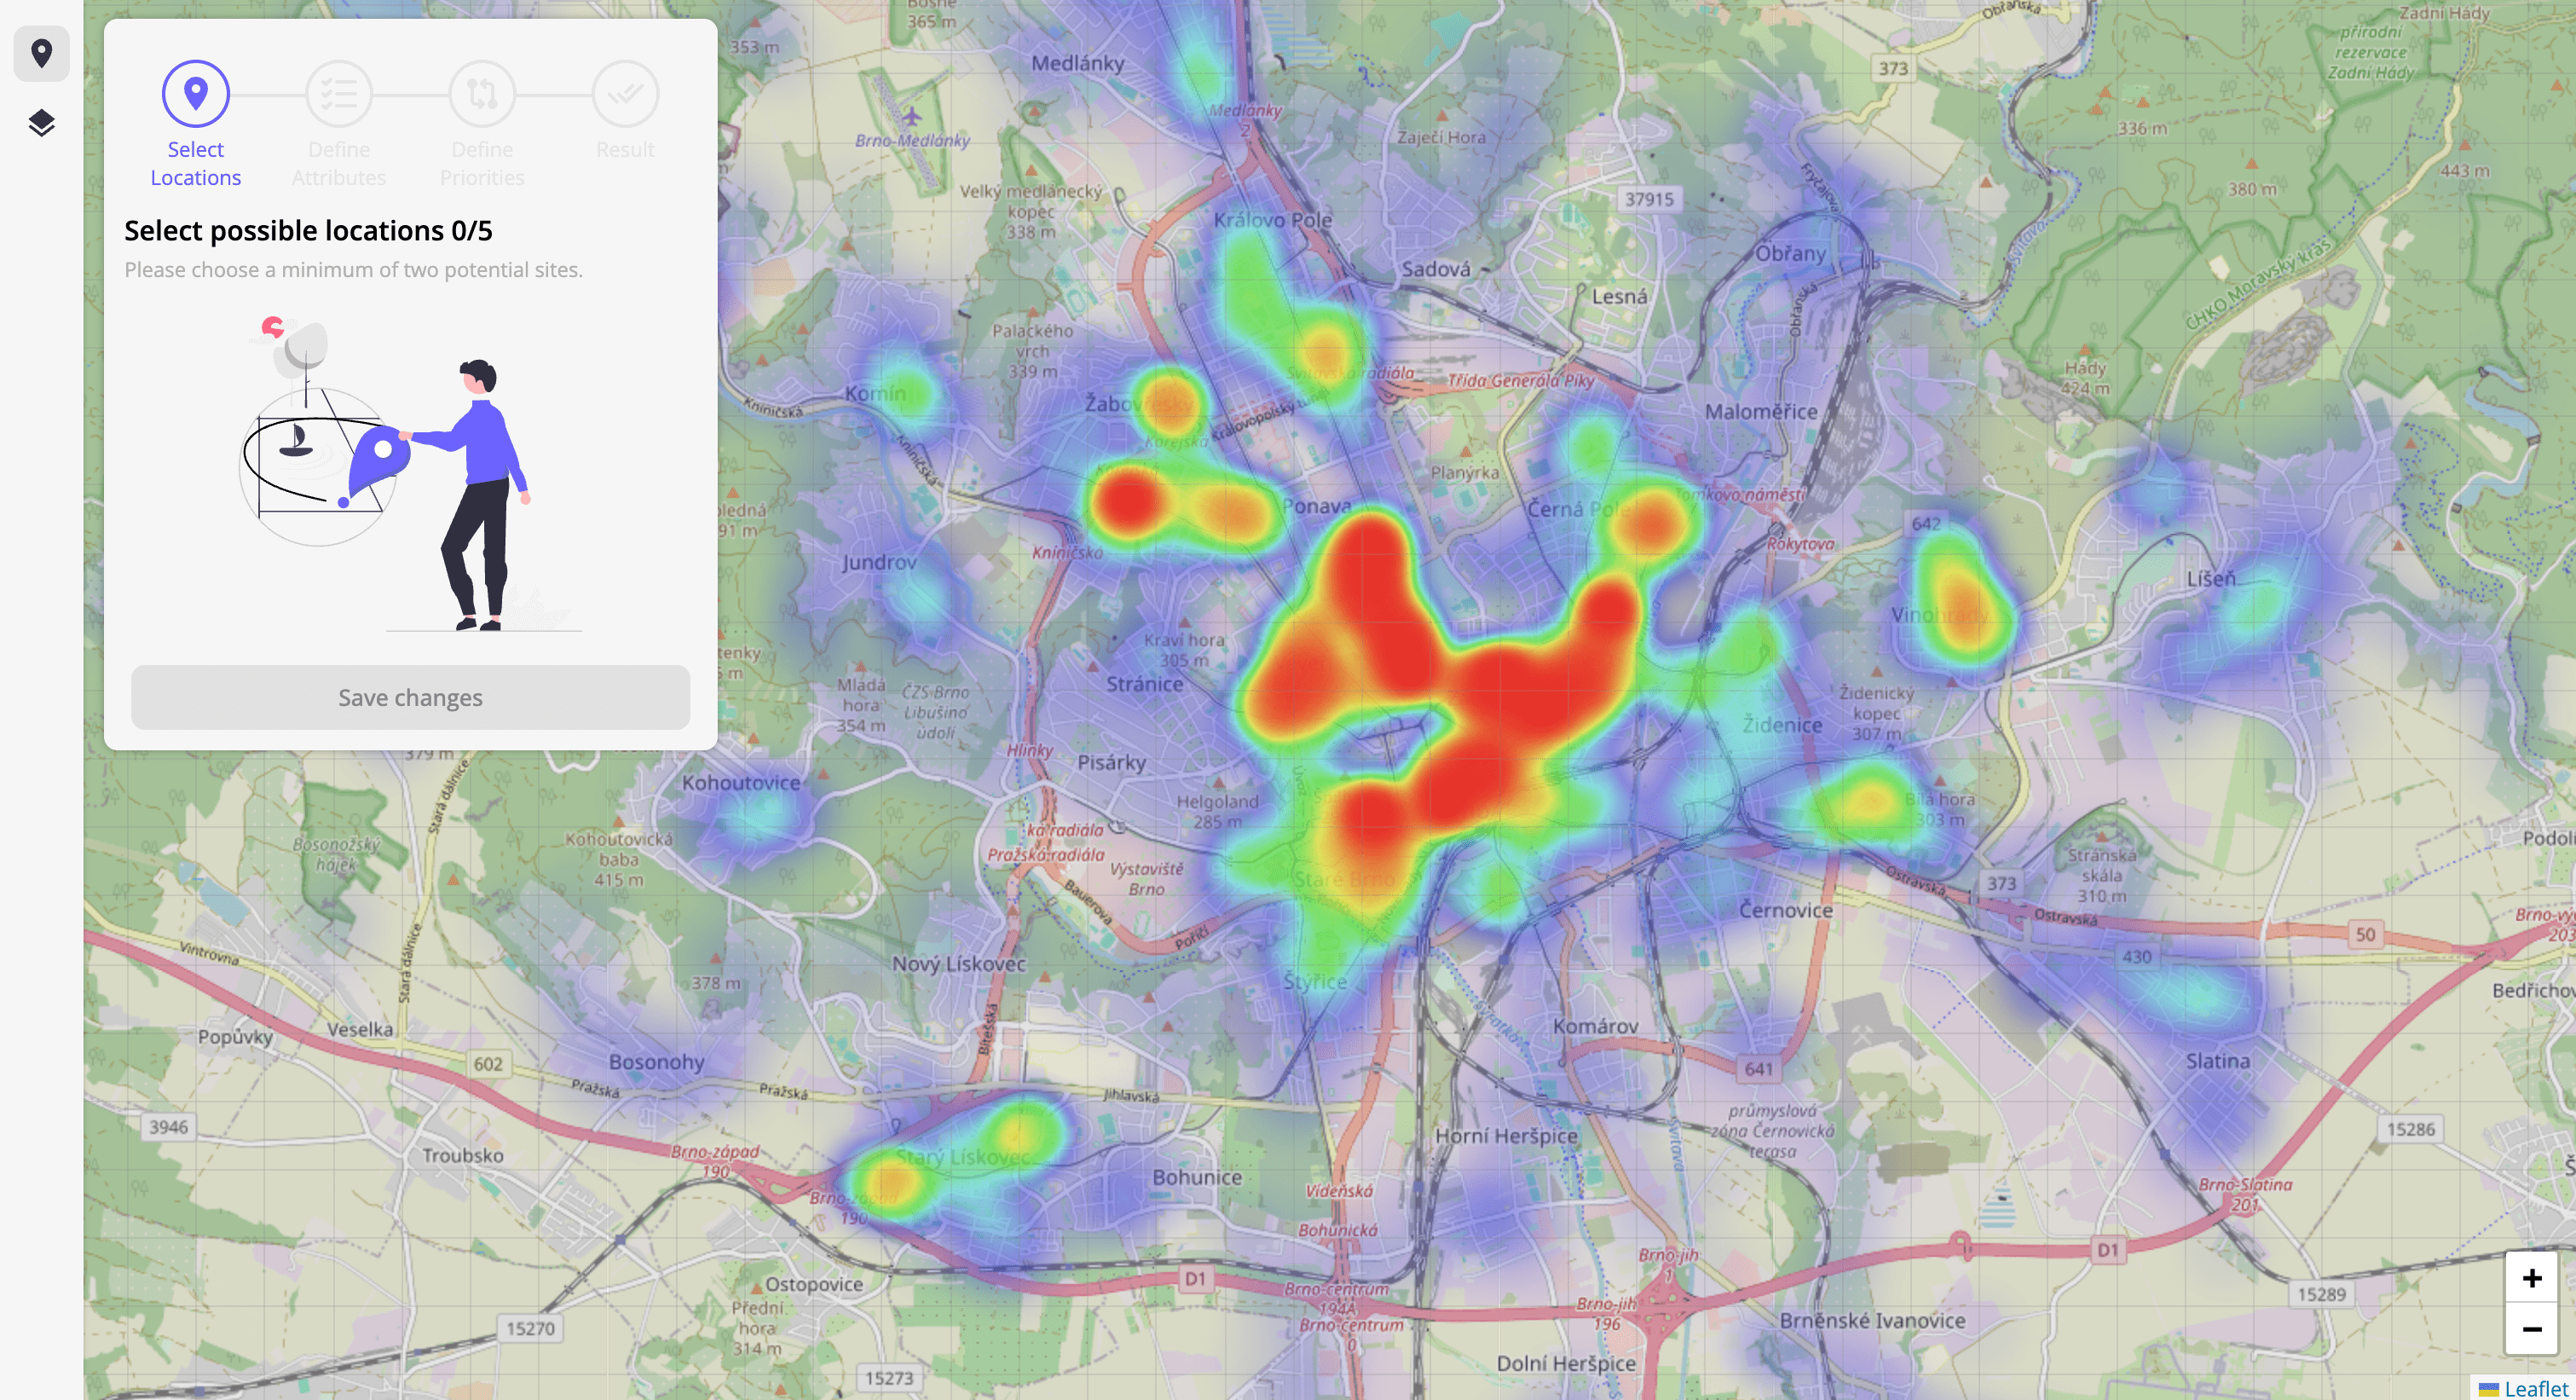
\includegraphics[width=1\linewidth]{obrazky-figures/ch6/map.png}
  \caption{Map}
  \label{fig:ui-map}
\end{figure}

The interactive map component itself is created and initialized using a customized \texttt{Map} class described in section \ref{subsec:extendedMap}. It is built-in inside of a custom hook \texttt{useMap} to provide a more natural way of interacting with it in React. For example, this hook exposes such methods as layer data fetching and layer toggling provided by the \texttt{Map}. Moreover, hook implements the state of a map to initiate re-render and reflect its changes in the \texttt{Map} component.

In order to track steps of the site selection process, map utilizes \texttt{enum SystemStatus} that contains such values as \texttt{SelectLocations}, \texttt{DefineAttributes}, \texttt{ScoreAttributes} and \texttt{Result}. Each value represents the step of a process, and based on this value, the map can display step-related information to the users and allow them to do certain actions that were described in section \ref{sec:idea}. 


While progressing through each step of the process, all step-related information is displayed within the \texttt{StepInfo} component, nested within a \texttt{MapInfo} component. Additionally, \texttt{Map} itself provides \texttt{MapContext} to access all the data from child components like \texttt{StepInfo} or \texttt{Layers}.

\subsection{Map Information}

The \texttt{MapInfo} serves as a top-left wrapper component responsible for generating nested components based on the current URL the user is accessing. Currently, there are two components that can be displayed within a \texttt{MapInfo}: \texttt{StepInfo} and \texttt{Layers}. Users can select these components from the left menu.

\subsection{Step Information}
\label{subsec:stepInfo}

The \texttt{StepInfo} component is a React component generated within a \texttt{MapInfo} component on a map (Figure \ref{fig:ui-stepinfo}). It presents information relevant to each step and includes buttons enabling users to advance to the next step or return to the previous one. When transitioning between steps, the \texttt{Map} component guarantees that all step-related data is preserved unless the user explicitly removes it.

To indicate the current step to the user, a \texttt{StepsContainer} component is employed as a wrapper for \texttt{StepInfo}. This container generates step-by-step components for each step, highlighting the current step accordingly. The state for this component is held by the \texttt{Map} and is accessed from its context.

\begin{figure}[ht]\centering
  \centering
  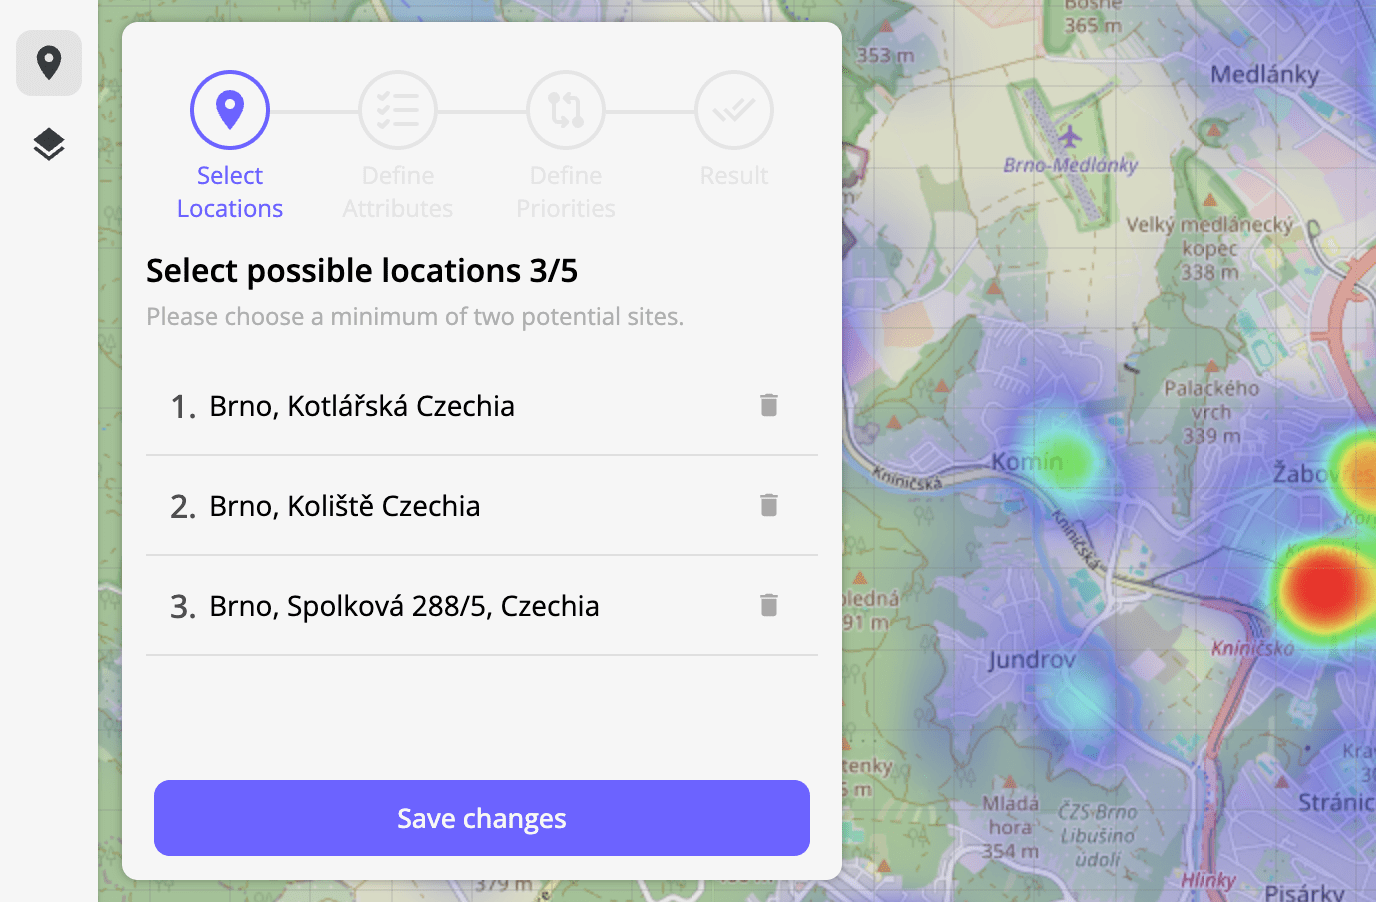
\includegraphics[width=0.8\linewidth]{obrazky-figures/ch6/mapinfo.png}
  \caption{Step information component}
  \label{fig:ui-stepinfo}
\end{figure}

\subsection{Layers}

The \texttt{Layers} component enables users to toggle the data layers sourced from the configuration file on the back-end. It provides information regarding the dataset currently in use and includes toggles for all available data layers (Figure \ref{fig:ui-layers}).

This component is accessible during any step of the process, it can provide extra information for the users when selecting possible locations.

\begin{figure}[ht]\centering
  \centering
  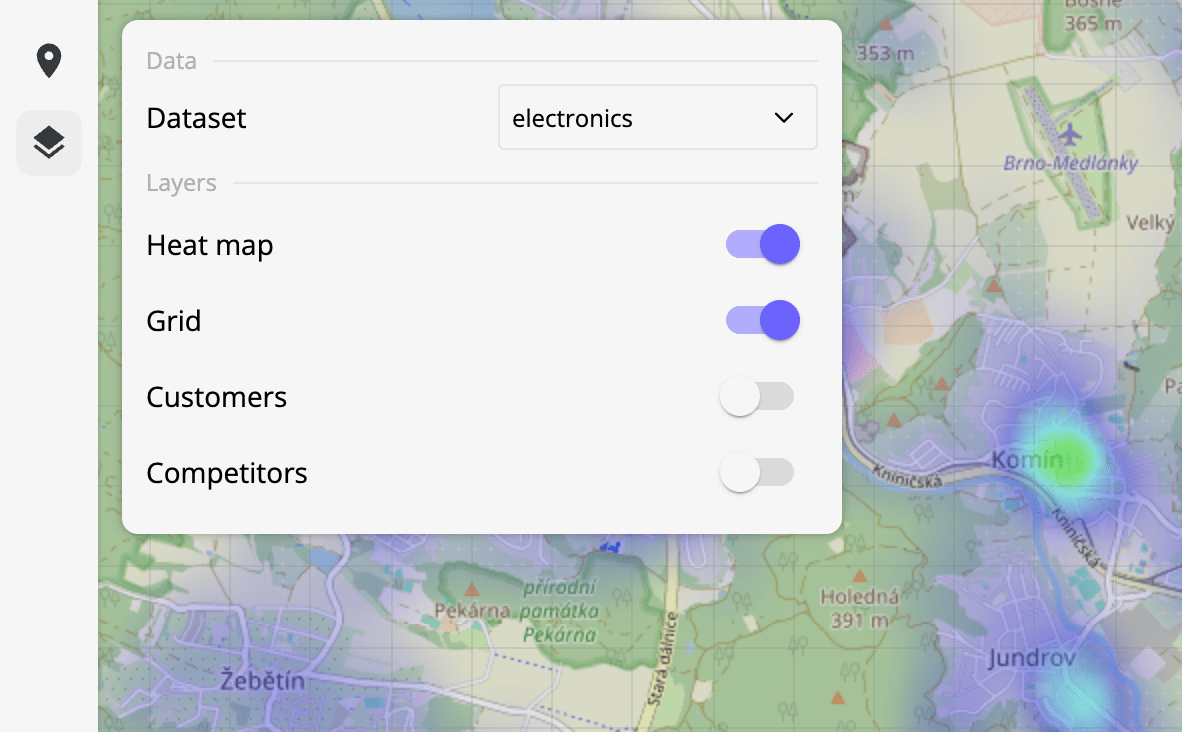
\includegraphics[width=0.8\linewidth]{obrazky-figures/ch6/layers.png}
  \caption{Layers component}
  \label{fig:ui-layers}
\end{figure}

\subsection{Modal Windows}

Modal windows are commonly utilized in this application to gather user input during various phases of the process, such as \texttt{DefineAttributes} and \texttt{ScoreAttributes}. Modal windows are effective for containing user inputs due to their ability to temporarily suspend the main workflow, thereby focusing user attention solely on the task at hand.

\subsubsection{Define Attributes Modal Window}

The \texttt{DefineAttributesModal} serves as a modal component employed within the\\ \texttt{DefineAttributes} step, where users are required to define a minimum of 2 features for potential outlets selected in the preceding \texttt{SelectLocations} step (Figure \ref{fig:uiModalDefineAttributes}). 

Within this modal window, users can define various attributes available to them. This implies specifying the attribute's name, value, and maximum value, which is essential for data normalization. While the default input format for all values is numeric, users have the flexibility to switch between quantitative and qualitative inputs if necessary.

\subsubsection{Define Score Modal Window}

Once the attributes are defined, they need to be compared. Utilized within the\\ \texttt{ScoreAttributes} step, the \texttt{DefinePrioritiesModal} component eases user interaction by enabling the comparison of attributes through sliders (Figure \ref{fig:uiModalDefineScore}). This modal window offers users a straightforward method to evaluate and prioritize attributes relative to each other.

\begin{figure}[ht]\centering
  \centering
  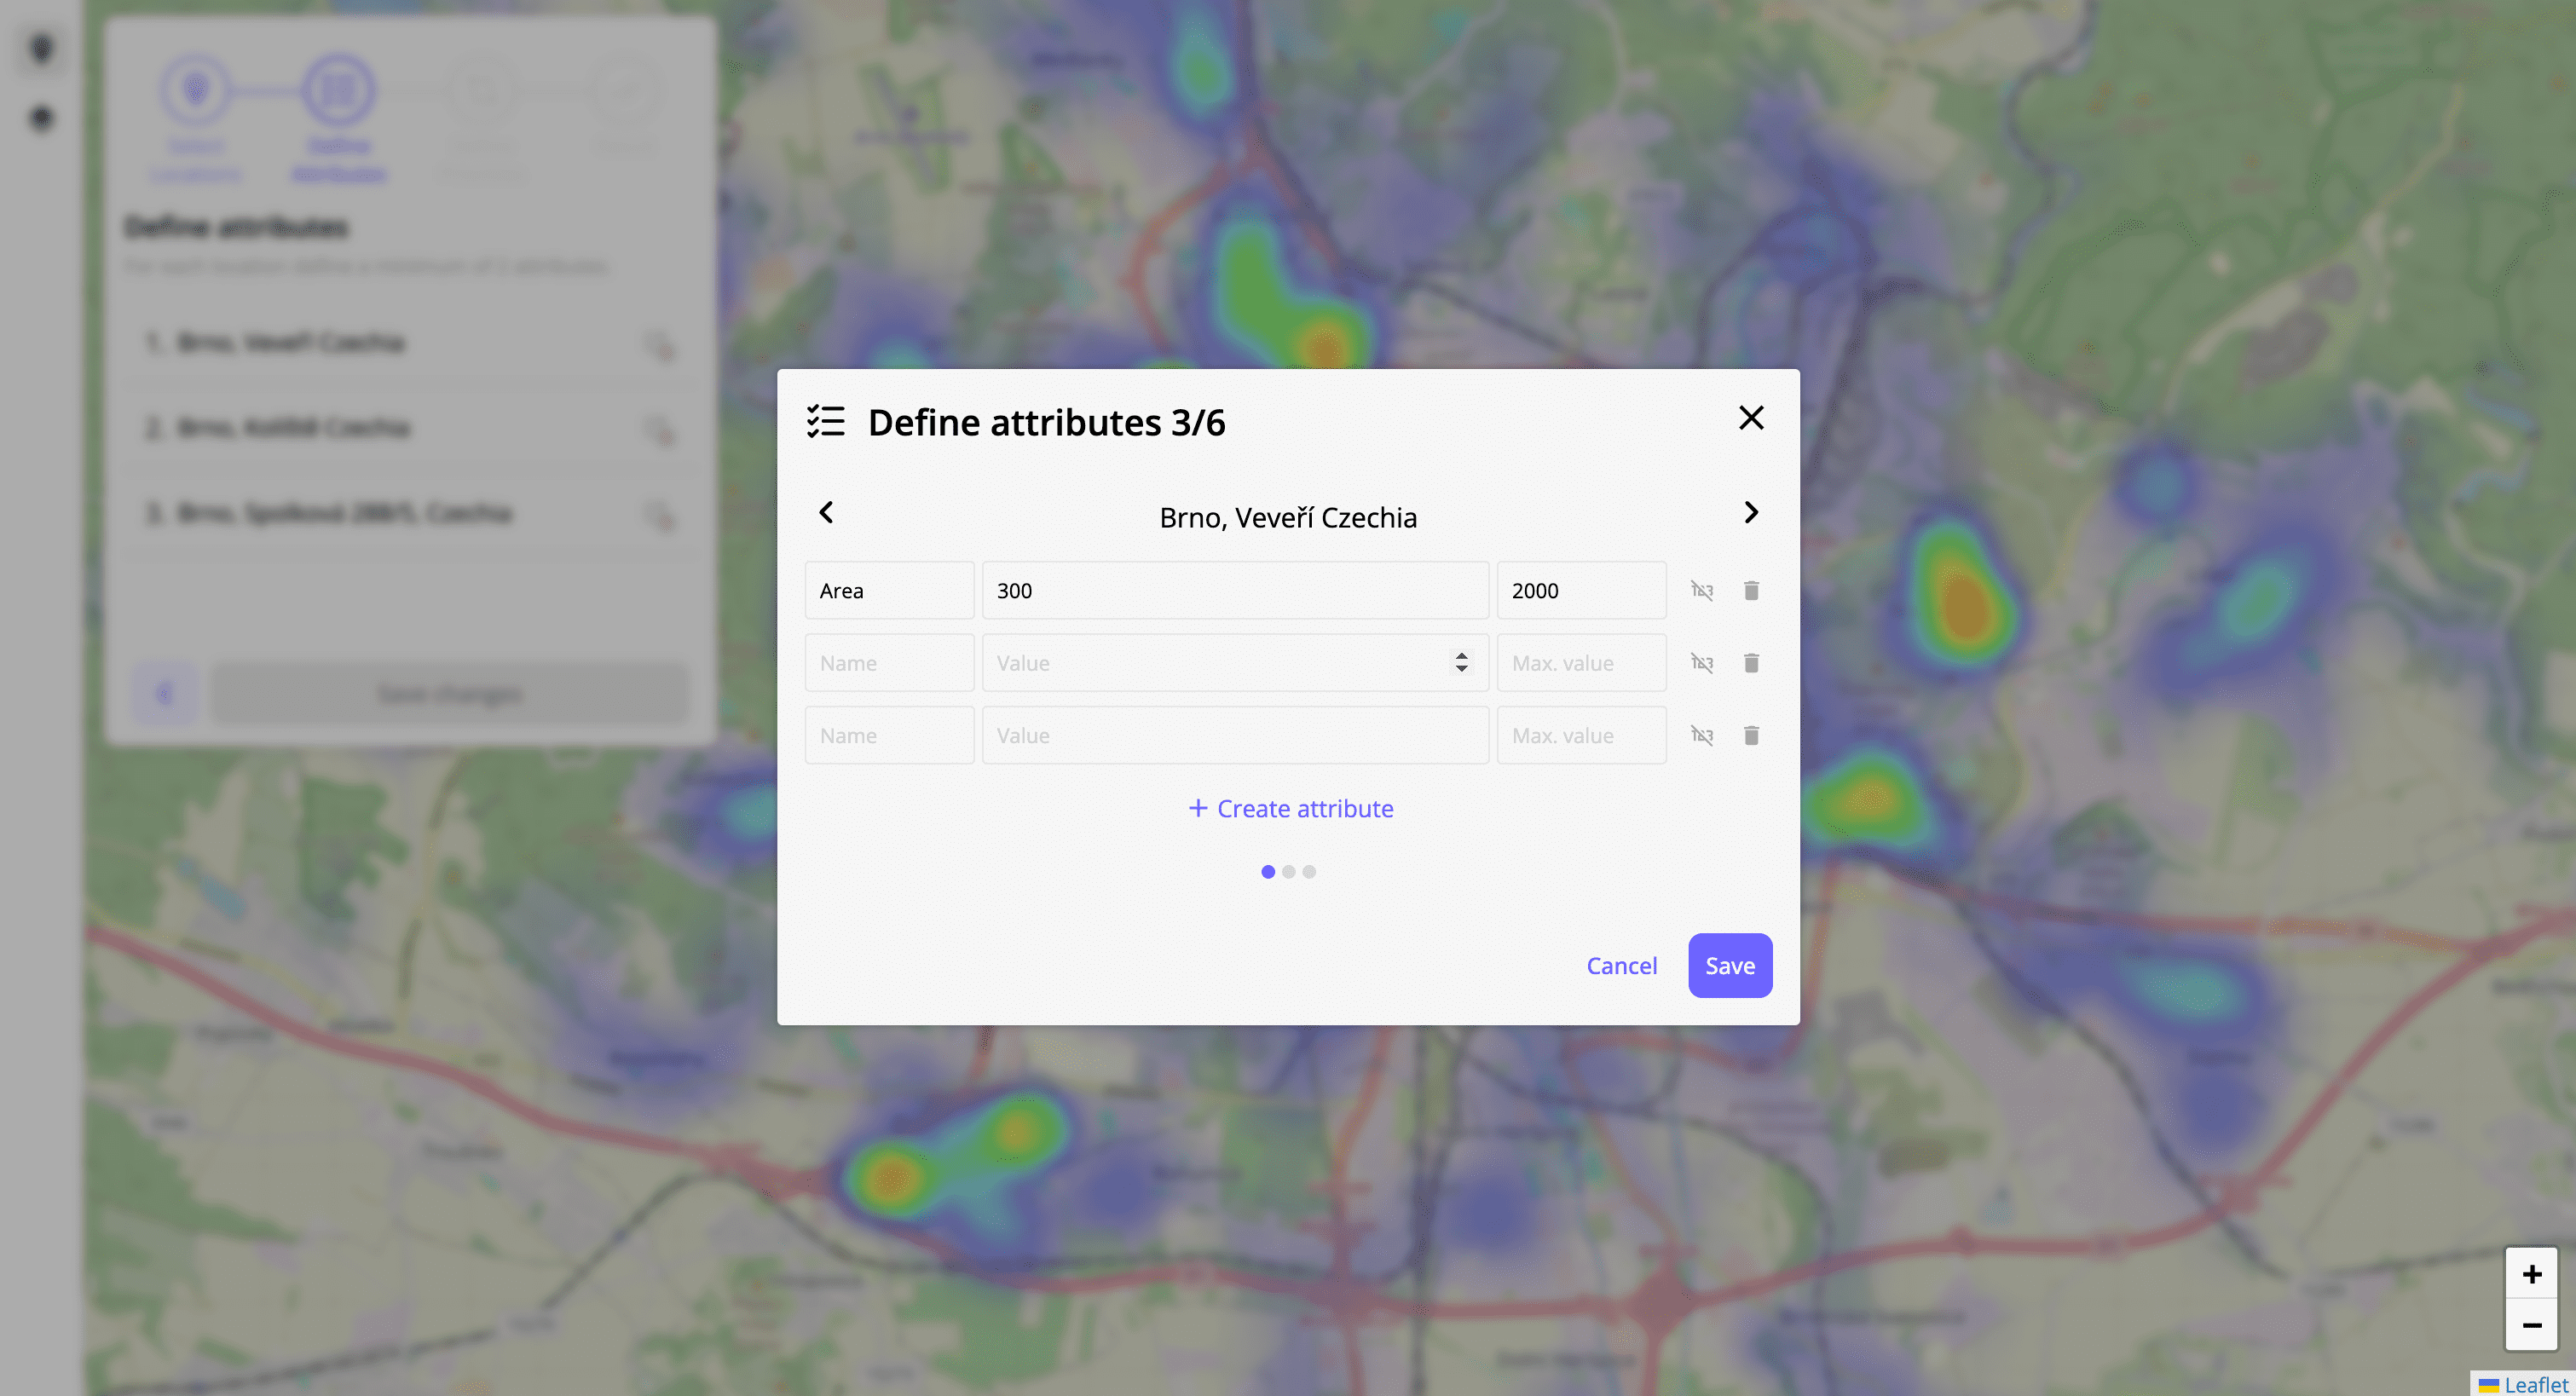
\includegraphics[width=0.8\linewidth]{obrazky-figures/ch6/attribute.png}
  \caption{Modal window to define attributes}
  \label{fig:uiModalDefineAttributes}
\end{figure}

\begin{figure}[ht]\centering
  \centering
  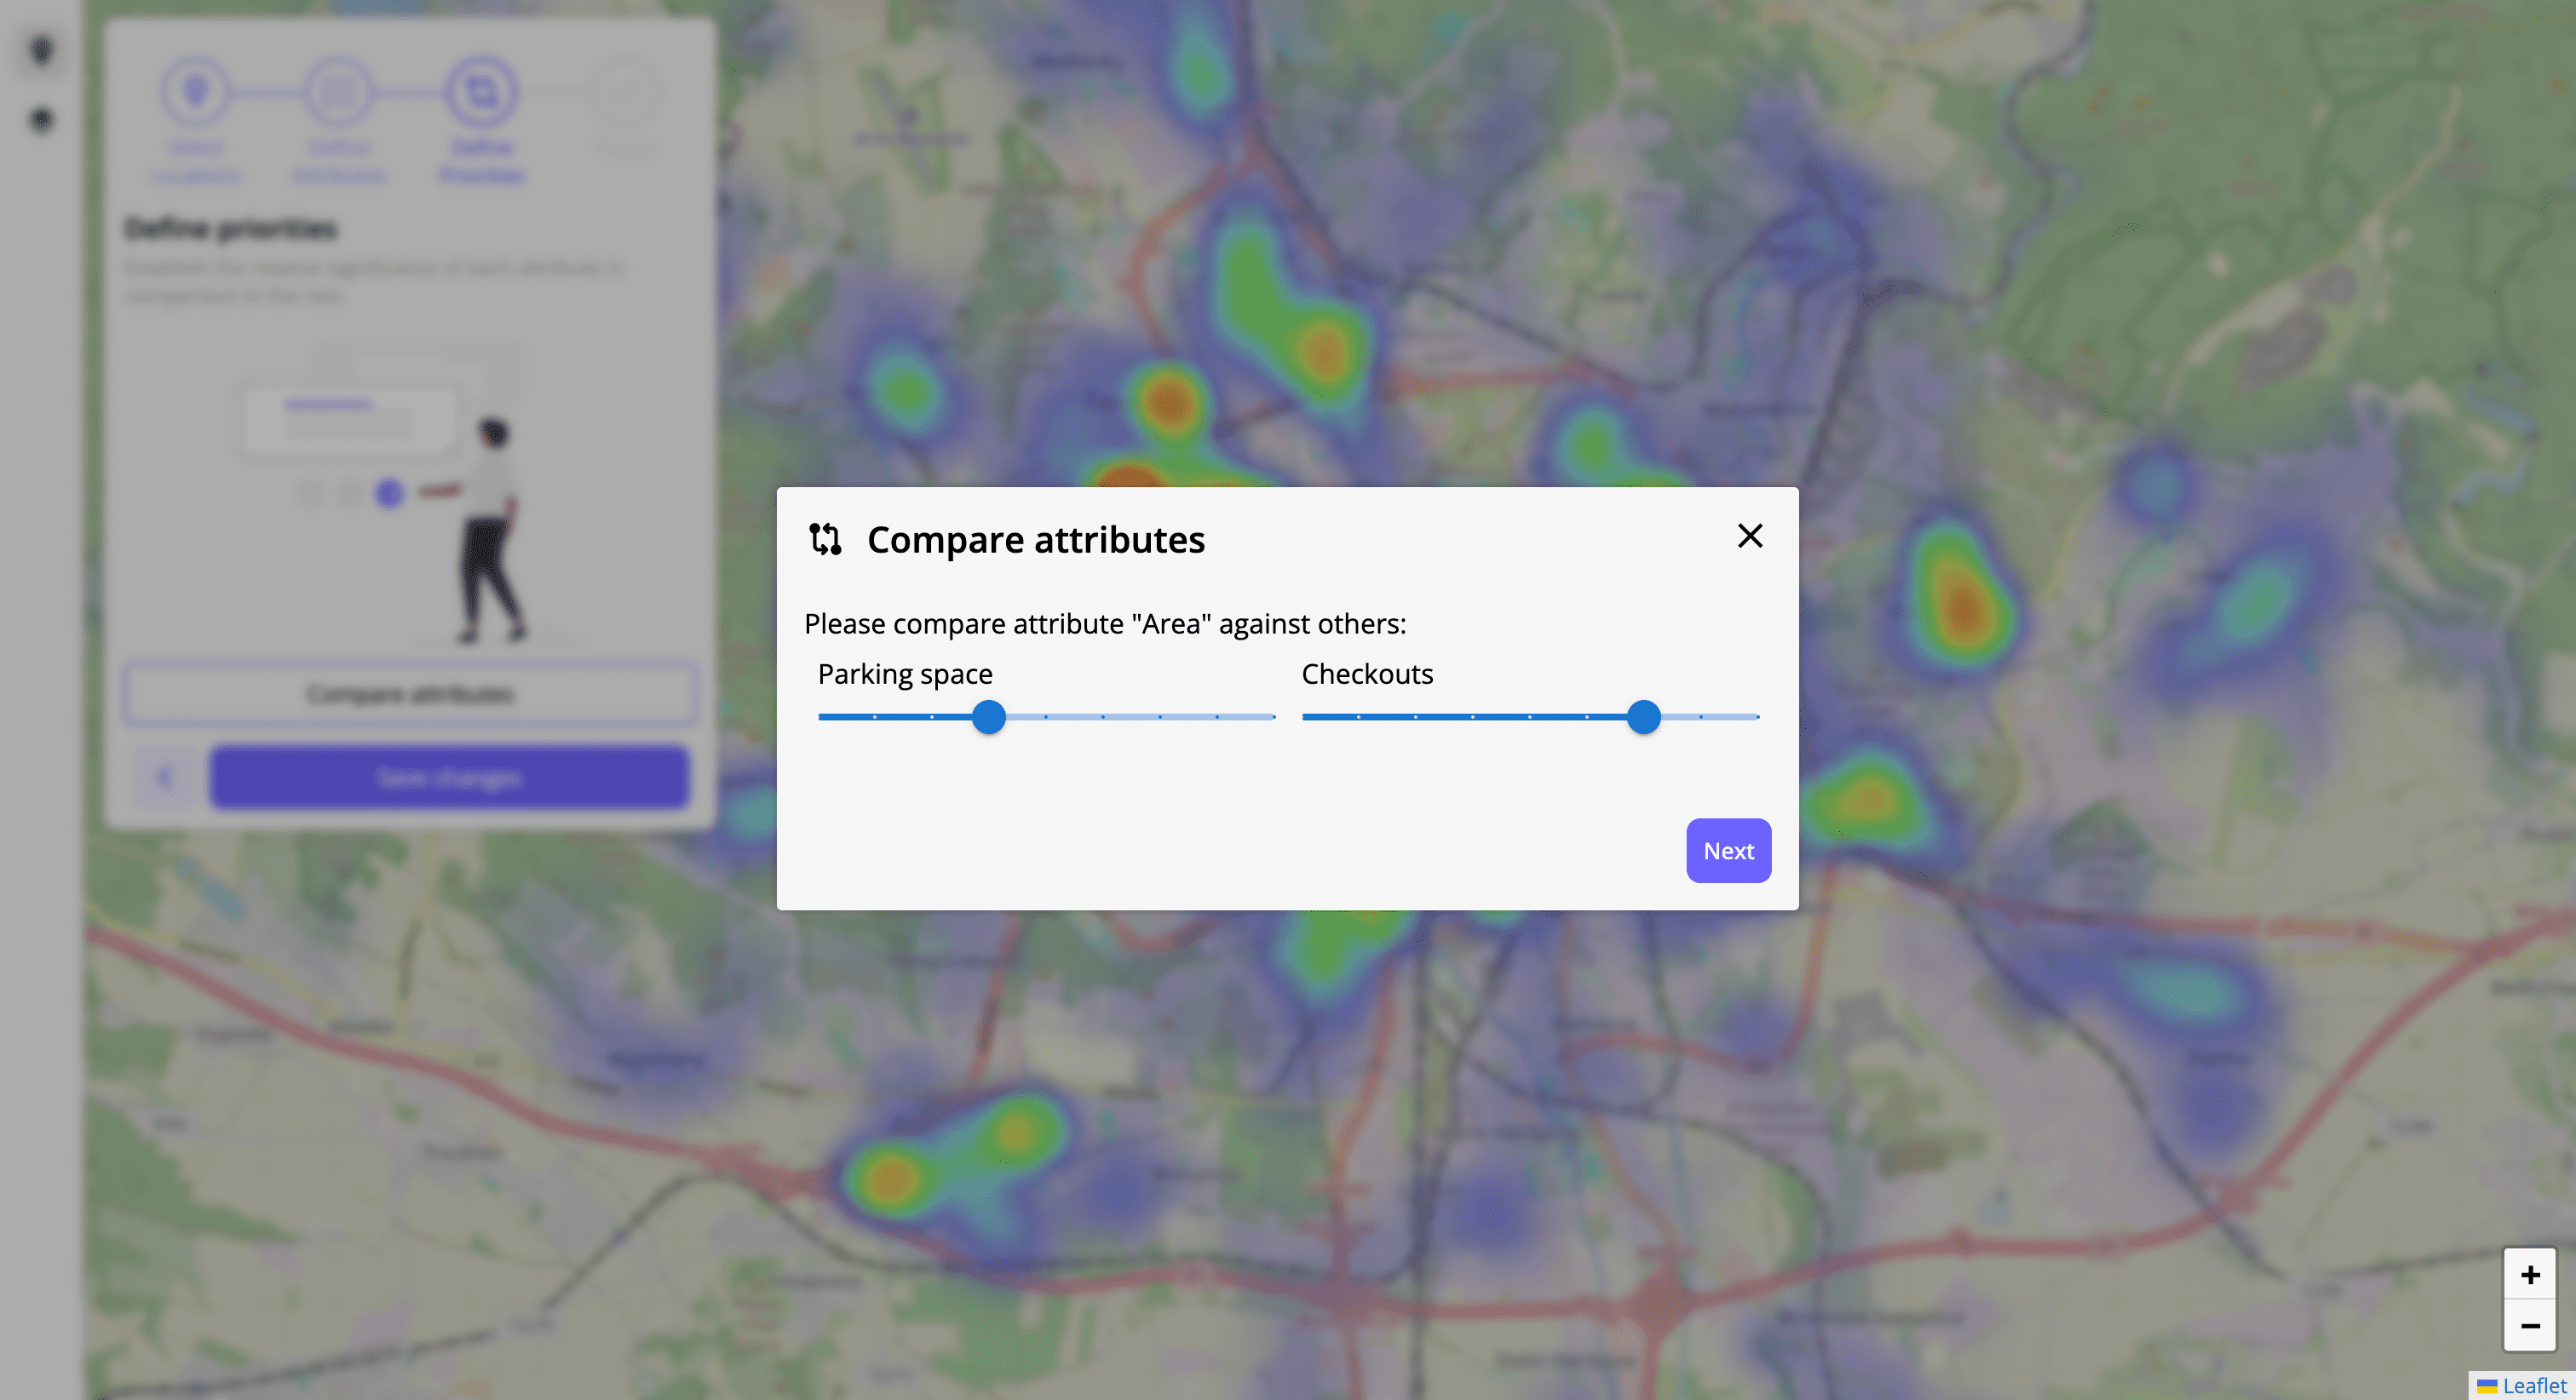
\includegraphics[width=0.8\linewidth]{obrazky-figures/ch6/compare.png}
  \caption{Modal window to compare attributes}
  \label{fig:uiModalDefineScore}
\end{figure}

\newpage

\section{Server Implementation}

The server functions as a standalone REST API application within the overall system architecture, developed in Python with the assistance of the FastAPI library. It can be configured with various regions or datasets, including customer data and competitor information, via a configuration file. The server implements the methodology described in Chapter \ref{ch:2}, and it exposes endpoints that expose specific information related to the current step of the process, which is controlled by the front-end client, as previously discussed in section \ref{implementation:front-end}.

\subsection{Configuration}
\label{section:configuration}

The configuration file for this application must be named \texttt{init.yaml}, and it must be located in the root folder of the server. In order for the server application to process this file, it must follow the structure:

\begin{itemize}
    \item \textbf{area}---The name of a region depicted on a map. It serves as the key for retrieving the path graph of the region prior to server initialization. The utilization of this graph will be described in Section \ref{subsec:highCompetitiveAreasCalculation}.
    \item \textbf{customers}---relative path to a dataset containing information about the number of individuals at specific addresses.
    \item \textbf{competitors}---a key-value structure of competitor datasets, where each key serves as the identifier for the dataset that users will see when choosing the business type.
    \begin{itemize}
        \item \textbf{path}---relative path to the server's folder pointing to a dataset that contains information about a certain category of competitors.
        \item \textbf{distanceDecay}---distance decay factor. This exponent was described in Section \ref{section:huff-model-calibration}. This property is optional, and the value is by default set to $1.75$\footnote{ArcGIS is a GIS system that has already implemented the Huff model. According to the ArcGIS documentation, the distance decay factor can range from $1.5$ to $2$---\url{https://pro.arcgis.com/en/pro-app/latest/tool-reference/business-analyst/understanding-huff-model.htm}} implicitly, but it can vary for every business category in different regions.
    \end{itemize}
\end{itemize}

Here is an example of a configuration file (Listing \ref{lst:config}). In this example, the distance decay factor was selected randomly.

\begin{lstlisting}[caption={Example configuration file.}, label=lst:config]
area: "Brno, Czech Republic"
customers: "./database/customers.json"
competitors:
  electronics:
    path: "./database/competitors-electronics.json"
    distanceDecay: 1.5
  grocery:
    path: "./database/competitors-grocery.json"
    distanceDecay: 2
  toys:
    distanceDecay: 2.5
    path: "./database/competitors-toys.json"
  ...
\end{lstlisting}


It is preferable for all datasets to correspond to the same geographic region. After completing the configuration process, the application can be initiated.

\subsection{Dataset Format}
\label{section:datasetFormat}

As was mentioned in section \ref{subsec:dataIntegration}, datasets that the user wants to integrate into this system must follow a specific format (Listing \ref{lst:dataFormat}).

\begin{lstlisting}[caption={Data format definition.}, label=lst:dataFormat]
[
    [latitude_1, longitude_1, data_1],
    [latitude_2, longitude_2, data_2],
    ...,
    [latitude_n, longitude_n, data_n]
]
\end{lstlisting}

\begin{itemize}
    \item \textbf{latitude}---latitude position of a point.
    \item \textbf{longitude}---longitude position of a point.
    \item \textbf{data}---associated information or data related to the corresponding latitude and longitude coordinates. For example, the number of customers or the size of a competitor.
\end{itemize}

Here is a simple example of the dataset with a number of people at specific addresses (Listing \ref{lst:exampleDataFormat}).

\begin{lstlisting}[caption={Example data with the list of latitude, longitude, and associated data that represent number of people.}, label=lst:exampleDataFormat]
[
    [49.177, 16.581, 4], 
    [49.164, 16.578, 5],
    ...,
    [49.166, 16.583, 49]
]
\end{lstlisting}

\subsection{High Competitive Areas Calculation}
\label{subsec:highCompetitiveAreasCalculation}

This section describes an implementation for determining regions with high competition. The methodology for this calculation was introduced in Section \ref{sec:determiningThePossibleLocations}.

The competitive areas calculation was implemented as a function \texttt{get\_geocompetition} located in the \texttt{/server/scripts/get\_geocompetition.py} file (Figure \ref{fig:competitiveAreasCalculationDiagram}).

The \texttt{get\_geocompetition} function is called whenever the server is launched in order to start the evaluation. It is important to mention that this function requires a graph provided by the \texttt{osmnx} library. It is installed before based on the specified region in the configuration and then used in the function in order to find distances between customers and competitors. It will be described further.

\begin{figure}[ht]\centering
  \centering
  \includesvg[width=1\linewidth]{obrazky-figures/ch6/competitive-areas.svg}
  \caption{Modal window to compare attributes}
  \label{fig:competitiveAreasCalculationDiagram}
\end{figure}

As an input, the function accepts paths to the customers and the competitors, and the distance decay factor is related to the type of the competitors. Both datasets follow the format defined in section \ref{section:datasetFormat}.

\subsubsection{Data Filtering}

The initial task within the function involves reading and transforming both datasets into \texttt{GeoDataFrames}. \texttt{GeoDataFrames}, offered by the geopandas library in Python, extend the functionality of pandas \texttt{DataFrame} to accommodate spatial data. A \texttt{DataFrame} in pandas is a two-dimensional, labelled data structure commonly used in Python for data manipulation and analysis. The data is organized into rows and columns. Each column can have a different data type. 

Following this conversion, data undergoes filtering processes, such as the removal of entries that are not located in the specified area. This may happen if the dataset covers a greater area than the server, because the borders which define the area on the server are fetched separately.

\subsubsection{Huff Model}

Once the data is filtered, the Huff model, which was described in Section \ref{section:huff-model}, is then applied. In the function, the Huff model was implemented in the following way:

\begin{itemize}
    \item Iterate through each competitor:
    \begin{itemize}
        \item Determine the nearest node to the competitor on the graph using method \\ \texttt{nearest\_nodes} provided by the \texttt{osmnx} library based on latitude and longitude coordinates.
        \item Iterate through each customer:
        \begin{itemize}
            \item Identify the nearest node to the customer on the graph using latitude and longitude coordinates.
            \item Compute the distance between the current competitor and the current customer utilizing the \texttt{shortest\_path\_length} method from the \texttt{networkx} library.
            \item Determine the travel time from the current customer to the current competitor.
            \item Calculate the probability of the current customer visiting the current competitor and append it to the list alongside other customers.
        \end{itemize}
        \item At this stage, a 2D array is formed where each index represents a competitor, and the element value denotes the probability of all customers visiting the competitor at the given index.
    \end{itemize}
    \item Convert the 2D array into a table where rows correspond to customers and columns correspond to competitors. For each competitor, compute the average probability of customer visits across all stores on the map (Table \ref{tab:customerCompetitorProbability}).
\end{itemize}

As a result, an array of averaged probabilities for all customers is obtained.

\begin{table}[htbp]
    \centering
    \begin{tabular}{|c|c|c|c|c|}
    \hline
     & \textbf{Competitor 1} & \textbf{Competitor 2} & \textbf{\dots} & \textbf{Competitor N} \\
    \hline
    Customer 1 & 0.08 & 0.06 & \dots & 0.05 \\
    Customer 2 & 0.06 & 0.05 & \dots & 0.07 \\
    Customer 3 & 0.07 & 0.06 & \dots & 0.06 \\
    \dots & \dots & \dots & \dots & \dots \\
    Customer N & 0.09 & 0.08 & \dots & 0.09 \\
    \hline
    \end{tabular}
    \caption{Example of 2D array of probabilities of $N$ customers visiting $N$ outlets.}
    \label{tab:customerCompetitorProbability}
\end{table}

\subsubsection{Kernel Density Estimation}

Once the array of averaged probabilities is obtained, it is time to apply kernel density estimation (KDE) to create a distribution of probabilities across the map. The KDE was introduced in the Section \ref{subsec:kde}. For the implementation, the library \texttt{scipy} was used. In order to create a smooth distribution, the \texttt{gaussian\_kde} was utilized.

\subsubsection{Grid-based Optimization}
\label{subsec:gridBasedOptimization}

Rather than computing the distance individually between each customer and competitor, I have used a grid-based approach, covering the entire map with cells measuring 500 meters each. By assigning competitors and customers to their respective cells, I simplified the process of calculating distances between cells. Leveraging this grid structure allowed for the efficient reuse of distances, particularly beneficial in scenarios where cells contained multiple competitors and customers.

\subsubsection{Dynamic Programming}
\label{subsec:dynamicProgramming}

The initial version of the \texttt{get\_geocompetition} function had significant potential for dynamic programming to simplify computations, particularly regarding tasks like calculating distances between nodes or finding the nearest node in the graph. I decided to cache the inputs and their corresponding results. This way, if the same input is encountered again in functions like \texttt{get\_nearest\_node} and \texttt{get\_distance\_to\_node}, the cached result can be returned directly, avoiding the need for redundant calculations.

\subsubsection{Caching Results}
\label{subsec:caching}

The performance of the function for identifying areas with high competition falls short of user expectations. While ideally, it should deliver results within seconds, as demonstrated in Section \ref{sec:performanceTesting}, the computations involved are extremely time-consuming. Even with the implementation of dynamic programming and optimization techniques, the fetching time for these computations remains prolonged, thereby impacting user experience negatively.

For this reason, I have decided to cache the results of the \texttt{get\_geocompetition} function. The cache will be stored in \texttt{/server/data} folder for future reuse, and if the user decides to rerun calculations, he is going to have to remove files with the cache. The cache has the same format as for datasets described in Section \ref{section:datasetFormat}.

In order to avoid situations in which the very first user needs to wait for computations, I have decided to launch estimation before the server startup so that the initial task of the server is to read all the datasets, perform all the calculations and save the result. In this case, the very first user will get a response instantly because the server is going to use cached results.

\subsection{Implementation of Analytic Hierarchy Process}

This section outlines the implementation of the Analytic Hierarchy Process (AHP), as detailed in Section \ref{subsec:ahp}. The AHP procedure is implemented within the function \texttt{ahp\_evaluate}, located within the \texttt{/server/scripts/ahp.py} file. This function is invoked during the final stage of the process to assess potential locations, considering both location attributes and attribute importance defined by the user.

To implement the Analytic Hierarchy Process, I have utilized the \texttt{Compare} method from the \texttt{ahpy}\footnote{AHPy---\url{https://github.com/PhilipGriffith/AHPy}} library. This method only requires parsing user comparisons into the appropriate format (Listing \ref{lst:ahp_dictionary}).

\begin{lstlisting}[caption={Example dictionary representing pairwise comparisons in the AHP process.}, label=lst:ahp_dictionary]
{
    ("Visibility", "Potential Market"): 1/4, 
    ("Visibility', "Accessibility by foot"): 4, 
    ("Potential Market", "Accessibility by foot"): 9
}
\end{lstlisting}

\subsection{API}

\begin{itemize}
\item \textbf{/test GET} Endpoint for testing purposes.
\item \textbf{/config GET} Retrieves configuration for the front-end application.
\item \textbf{/customers GET} Returns dataset of customers.
\item \textbf{/competitors POST} Returns dataset of competitors by category name.
\item \textbf{/area POST} Calculates and returns areas with a high competition.
\item \textbf{/result POST} Calculates the resulting list of locations with ratings based on user input.
\end{itemize}

\subsection{Documentation}

I have decided to utilize Swagger\footnote{Swagger---\url{https://swagger.io/}} for documenting my endpoints because of its integration with FastAPI. Swagger automatically generates interactive API documentation based on the defined FastAPI endpoints. This ensures that the API documentation stays up-to-date with the codebase without manual intervention, saving time and effort (Figure \ref{fig:swagger}).

\begin{figure}[ht]\centering
  \centering
  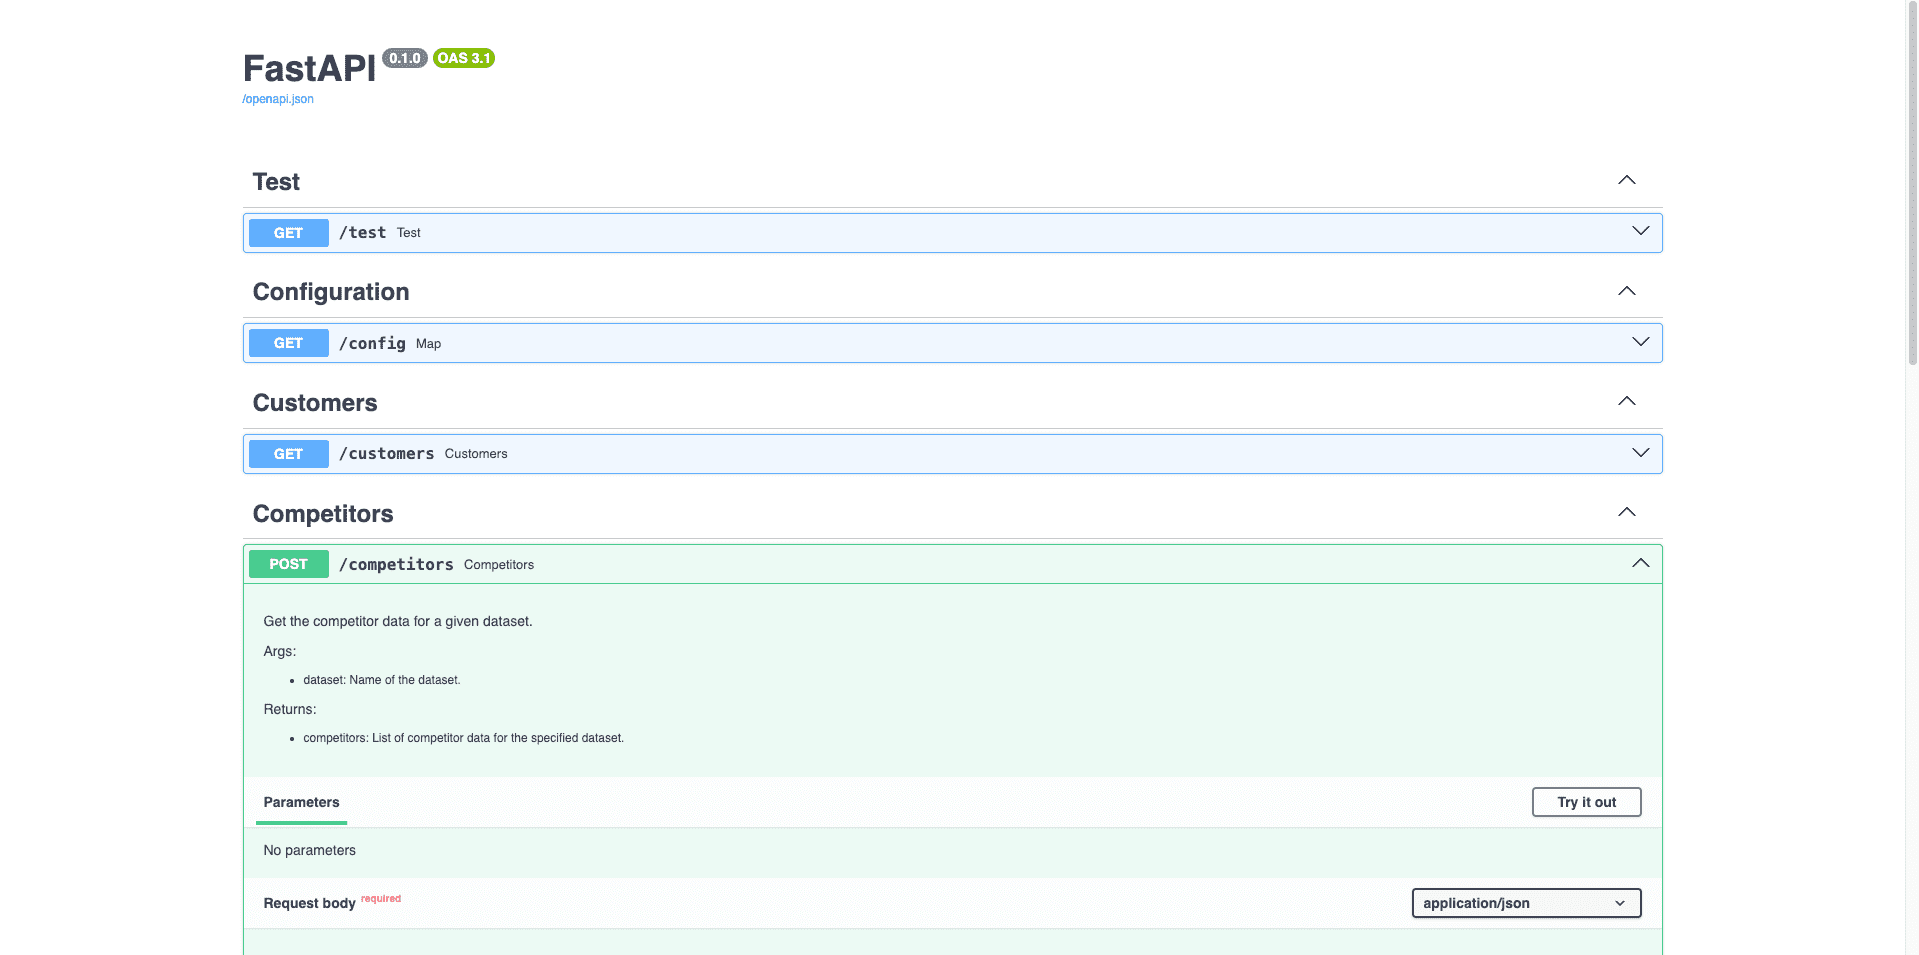
\includegraphics[width=1\linewidth]{obrazky-figures/ch6/swagger.png}
  \caption{Screenshot of swagger documentation for the server.}
  \label{fig:swagger}
\end{figure}